\documentclass[border=2pt]{standalone}
\usepackage{pgfplots}
\usetikzlibrary{arrows.meta}
\pgfplotsset{compat=1.18}
\begin{document}
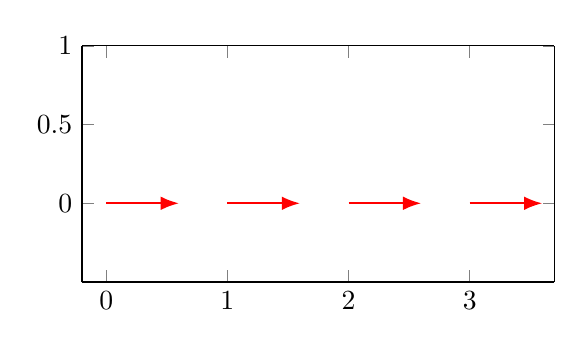
\begin{tikzpicture}
\begin{axis}[view={0}{90},scale only axis,width=6cm,height=3cm,
  xmin=-.2,xmax=3.7,ymin=-.5,ymax=1,zmin=-1,zmax=1,enlargelimits=false,
  xtick={0,1,2,3},ytick={0,.5,1},domain=0:3,samples=4,
  y domain=.4:.8,samples y=1]
  \addplot3[red,thick,-{Latex},quiver={u=.6,v=0}] {0};
\end{axis}
\end{tikzpicture}
\end{document}
